\section{推理}

\begin{quotation}
\textit{推理是逻辑学的实践应用,通过系统化的思考方法和训练,我们能够解决复杂问题并发展批判性思维能力。}
\end{quotation}

如前所述,逻辑学是研究用于区分正确推理与不正确推理的方法和原理的学问。\textbf{推理}与\textbf{论证}都是从已知的(或为了某种目的而肯定的)前提推出结论的过程。至此,我们一直在分析和评估的是别人的论证。当然,我们在决定自己应如何行动、评价他人的行动、为道德的或政治的信念进行辩护等方面,我们每天都要建构我们自己的论证。建构和运用好的论证之技能是有巨大价值的。

推理的技能可以通过训练来提高。为了促进这样的训练,许多推理游戏(例如国际象棋、围棋、Mastermind ${ }^{(1)}$ 等)都是极好的手段。而那些用以强化和测试我们的逻辑技能的推理谜题,也无疑是相当实用的。推理不仅是一项必要的活动,也是一项愉快的活动——当我们解决了为提高技能和使人娱乐双重目的而设计的一些逻辑问题时,它所产生的乐趣是不言而喻的。

人为设计的问题比现实生活中的问题更简洁,通常也更简单。但是解答它们是具有挑战性的,经常需要锲而不舍地反复推理,这在思考模式上与侦探或新闻工作者或陪审员没有很大不同。可能需要找到一个推理系列,在这个系列中,所得的次结论被用做后来推理的前提。也可能要求具有一定的洞察能力,要找到解决问题的路径需要对早先假设或发现的信息进行创造性的重组。解决人为设计的问题往往是比较困难的,有时会无功而返,但是当通过推理的成功应用解决了问题时,是非常令人满足的。逻辑游戏和谜题解答,伴随各种推理模型的运用,都是很好的娱乐。"对思虑的享受",美国哲学家约翰•杜威写道,"是受过训练的大脑的标志"。

\footnotetext{(1)种著名的网络智力游戏。
}

\subsection{推理问题的类型与解法}

推理问题的一个常见类型是智力测验,仅仅使用所提供的线索,我们被要求理清和辨识有关的几个人物的名宁,或角色,或其他事实。下面是一个比较简单的例子:

\begin{displayquote}
在某个航班的全体乘务员中,飞机驾驶员、副驾驶员和飞行工程师的职务由爱伦、布朗和卡尔三人担任,但不必是这个次序。\\
副驾驶员是个独生子,钱挣得最少。\\
卡尔与布朗的姐姐结了婚,钱挣得比驾驶员多。\\
问:三个人每人担任什么职务?
\end{displayquote}

为了解答这样的问题,我们首先要寻找一个范围,在这个范围中我们有足够的信息去得到超出前提所给信息的一些结论。我们从前提中知道许多关于卡尔的情况:他不是飞机驾驶员,因为他挣得比驾驶员多;他也不是副桇驶员,因为副驾驶员挣得最少。通过排除我们可以推出,卡尔一定是飞行工程师。

使用上述的次结论,我们可以确定布朗的职务。布朗不是副驾驶员,因为他有一个姐姐而副驾驶员是个独生子;他也不是飞行工程师,因为卡尔是飞行工程师。所以布朗一定是飞机驾驶员,而仅剩的爱伦一定是副驾驶员。

\subsection{矩阵分析法}

在解答这类问题(有时非常复杂)时,建构一个备选项的图示是非常有帮助的,这种图示叫做\textbf{矩阵},当我们积累了新的信息时就把它填人表中。要见识这种矩阵图的作用,请考虑下面的问题:

\begin{displayquote}
阿伦佐、库特、鲁道夫和威拉德是四个天资极高的创造性的艺术家。一个是舞蹈家,一个是画家,一个是歌唱家,一个是作家,但不必是这个次序。\\
(1)那天晚上歌唱家在音乐会舞台上进行他的首次演出时,阿伦佐和鲁道夫在观众席上。\\
(2)库特和作家两人有画家为他们画的生活肖像。\\
(3)作家正准备写一本阿伦佐的传记,他写的威拉德的传记是畅销书。\\
(4)阿伦佐从未听说过鲁道夫。\\
问:每个人的艺术领域是什么?
\end{displayquote}

将这些前提中断定的许多事实记在头脑中,也记住几个可以从这些前提推出的分结论,这是一项必需的工作。把我们的推论记在便条上可能是有帮助的,但是也可能导致混淆和零乱。我们需要一种有效方法,来贮备已知的信息和所引出来的中间结论,能把已知的信息和推出的信息整齐地记录下来,并随着推论的数目不断增长以及论证的链条不断拉长供我们使用。而在我们要建构的矩阵表中就有空间去表示所有相关的可能选择,并能记录下每一个引出的推论。

这个问题的矩阵表必须是显示这四个人(用四行表示)和他们从事的四种艺术职业(用四列表示)的一个列阵,如下所示:

\begin{center}
\begin{tabular}{|l|l|l|l|l|}
\hline
 & 舞蹈家 & 画家 & 歌唱家 & 作家 \\
\hline
阿伦佐 &  &  &  &  \\
\hline
库 特 &  &  &  &  \\
\hline
鲁道夫 &  &  &  &  \\
\hline
威拉徳 &  &  &  &  \\
\hline
\end{tabular}
\end{center}

当我们断定名字在某行左边的人不可能是从事某列顶端所示职业的艺术家时,我们就在那个人名字的右边以那个职业做标题的列中空格写一个 N (代表"no",或写一个"一"符)。我们立即可以从前提(1)做出推断,阿伦佐和鲁道夫都不是歌唱家,所以我们在第三列(歌唱家)他们名字的右边空格写上一个 N。同样,我们可以从前提(2)推断库特既非画家也非作家,所以我们把一个 N 记在第二列(画家)和第四列(作家)他的名字右边的空格中。从前提(3)我们看出作家既非阿伦佐也非威拉德,所以我们把 $N$ 记在第四列他们名字右边的空格中。至此我们记录的所有项目都得到了原先所给信息的证明,现在的矩阵表如下:

\begin{center}
\begin{tabular}{|l|l|l|l|l|}
\hline
 & 舞蹈家 & 画家 & 歌唱家 & 作家 \\
\hline
阿伦佐 &  &  & N & N \\
\hline
库 特 &  & N &  & N \\
\hline
鲁道夫 &  &  & N &  \\
\hline
威拉德 &  &  &  & N \\
\hline
\end{tabular}
\end{center}

从已获得的信息我们可以用排除法断定,鲁道夫一定是作家,所以我们在第四列(作家)下鲁道夫名字右边的空格中记一个 Y(代表"yes",或记一个"+"符)。现在从列阵看,很明显,画家一定或是阿伦佐或是威拉德,并且我们在这里可以排除阿伦佐:鲁道夫有画家给他画的肖像(从前提(2)可知),阿伦佐从未听说过鲁道夫(从前提(4)可知),因此阿伦佐不可能是画家。这样我们记一个 N 在第二列(画家)阿伦佐名字右边的空格中。

接着我们可断定阿伦佐一定是舞蹈家,从而在第一列(舞蹈家)阿伦佐名字右边的空格记一个 Y。现在我们可以在舞蹈家列中为库特和威拉德二人分别记人一个 N 。对库特来说剩下的唯一可能是歌唱家,所以我们记一个 Y 在那个空格中,并且记一个 N 在威拉德名字右边歌唱家列的空格中。再通过排除我们断定,威拉德一定是画家,并将一个 Y 填入矩阵表的最后一个空格。完成的图示是这样的:

\begin{center}
\begin{tabular}{|c|c|c|c|c|}
\hline
 & 舞蹈家 & 画家 & 歌唱家 & 作家 \\
\hline
阿伦佐 & Y & N & N & N \\
\hline
库 特 & N & N & Y & N \\
\hline
鲁道夫 & N & N & N & Y \\
\hline
威拉德 & N & Y & N & N \\
\hline
\end{tabular}
\end{center}

从这个填满的矩阵表中我们可以得到答案:阿伦佐是舞蹈家,库特是歌唱家,鲁道夫是作家,威拉德是画家。

当要求提供几种不同范围的答案时,这种综合性质的智力游戏就变得更复杂了。有些这样的问题非常具有挑战性,并且不使用矩阵方法几乎不可能解决。 ${ }^{[53]}$

另一些推理问题提出的是一种不同的挑战。下面是一个精致、娱人但不是很困难的问题。在阅读紧随其后的答案之前请努力解决它。

你面前有六个球:两个红球、两个绿球和两个蓝球。在每一对同色球中,你知道其中一个比另一个重。你还知道所有三个重球的重量相同,所有三个轻球也一样重。另外,这六个球(把它们分别叫做 R1、R2、G1、 G2、B1 和 B2)难以区分。你只有一架天平秤盘。

问:若在秤盘上称量不能超过两次,如何能辨认出所有三对球中的重球和轻球?

\section*{答案:第一次称量: $\mathbf{R 1 + G 1 / / R 2 + B 1}$}
如果两边平衡:R1 和 R2一对红球中,一个重一个轻。因两个红球分别在秤盘的两边,我们知道如果两边平衡,那么每一边的另一个球一定也是一重一轻——因为如果两个重球在同一边,这一边就一定沉下去。因此,我们知道两者必居其一:G1 重而 B1 轻,或者 G1 轻而 B1 重。

如果在第一次称量时两边平衡,那么第二次称量:G1//B1。无论这一次称量的结果是什么,所有球的轻重都可以辨认出来。

如果(在这次称量中)G1 沉下去,那么:\\
-G1 重(且 G2 轻),且\\
-B 1 轻(且 B 2 重),且\\
$\cdots \mathrm{R} 1$ 轻(且 R2 重)。\\
如果(在这次称量中)G1 升上去:(上述结论的)反面就是真的。\\
但是,倘使在第一次称量中 $(\mathrm{R} 1+\mathrm{G} 1 / / \mathrm{R} 2+\mathrm{B} 1)$ 两边不平衡将会怎样?假设 $\mathrm{R} 1+\mathrm{G} 1$ 沉下去。(如果 $\mathrm{R} 1+\mathrm{G} 1$ 升上去,随之答案就简单地倒转过来。)

我们知道在这种情况下 R1(在这一边的红球沉下去)一定是重的;因为如果 R1 是轻的,R2 就是重的;并且如果 R2 是重的,R1+G1 就不会沉下去。

因为 R1 是重的,下面三种联合体之一一定是如此这般:\\
(a)G1 是轻的,并且 B 1 是轻的;或者\\
(b)G1 是重的,并且 B 1 是重的;或者\\
(c)G1 是重的,并且 B1 是轻的。

\section*{如果 $\mathbf{R 1 + G 1 ~}$ 在第一次称量中沉下去,第二次称量: $\mathbf{R 1 + R 2 / /}$ $\mathrm{G} 1+\mathrm{B} 1$ 。}
我们已经知道 R1 是重的。在这第二次称量中,R1+R2(重 + 轻)一定是下列两种情况之一:沉下去或升上去,或者两边平衡。无论是哪一种结果,我们都可以辨认出所有球的轻重如下:\\
(x)如果 R1+R2 沉下去,G1 和 B1 一定都是轻的(因为一个重的加一个轻的会在重量上超过仅仅两个轻的相加)。在这种情况下联合体一定是上面的(a)型:G1 是轻的且 B1 是轻的一一所有问题都被解决。\\
(y)如果 R1+R2 升上去,G1 和 B1 一定都是重的(因为重+轻在重量上只能被两个重的相加超过)。在这种情况下联合体一定是上面的(b)型:G1 是重的且 B1 是重的——所有问题都被解决。\\
(z)如果两边平衡,G1 和 B1 也一定是重+轻。在这种情况下联合体一定是上面的(c)型:G1 是重的且 B1 是轻的一一所有问题都被解决。

将这个问题推荐给你的朋友们之前,请练习说明上述答案!\\
在现实世界中,我们经常被要求从某个当前事态推出它的起因,从事

情现在是什么推出其过去是什么。科学家——特别是考古学家、地质学家、天文学家、医学家——通常面对着探究其起源的事件或条件。企图说明事情为何从过去的状况发展到现在的状况的推理叫做回溯分析。例如,令天文学家惊奇的是,1996年在地球旁边疾驰而过的彗星海库塔克(Hy- akutake)放射出比任何一位科学家曾预言的一颗彗星能够放射出的强 100倍的可变 X 射线。德国马克斯-普朗克研究所的一位彗星专家评论说: "为了研究这些数据,我们中断了我们正在进行的工作——但这是一种你喜欢拥有的问题。"

我们确实喜欢拥有这样的问题。因此,回溯分析问题经常是为娱乐而设计的。然而这样的问题也有一种特殊的困难:由科学的或历史的知识提供的现实世界的逻辑框架一定是以某种方式由问题自身规定的。一些规则或规律一定是在逻辑分析能够进行的范围内提出的。

棋盘是一种最著名的回溯分析问题的装置,而下棋规则规定了必要的 63 理论语境。下棋无须什么技术,但对(国际)象棋规则不熟悉的读者可以跳过如下例示。

象棋中的回溯问题通常采取这样的形式:棋盘中棋子的安排是给定的,对一局棋赛进行回溯分析,以比赛中遵守了所有比赛规则为前提。例如,图 1-1 代表一局棋赛所得到的形势,比赛中所有的着数都与象棋规则一致。那么,刚刚走的一着棋或几着棋是什么?\\
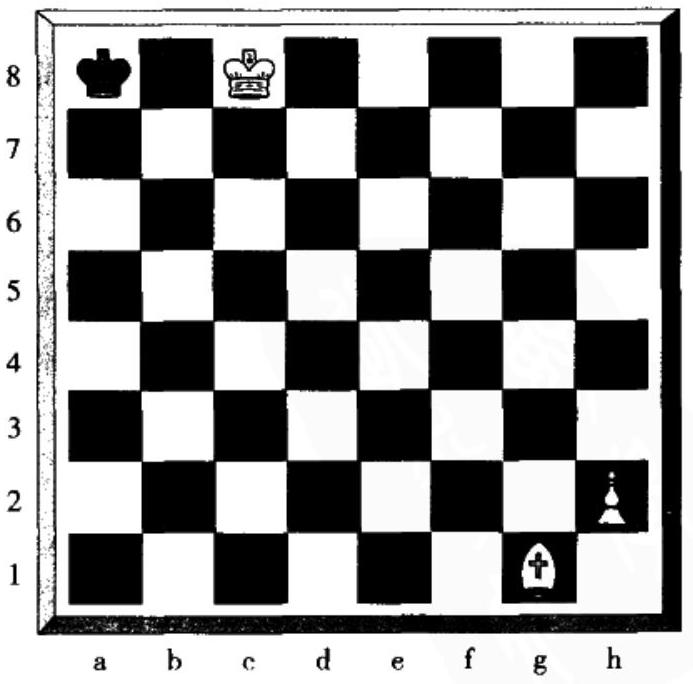
\includegraphics[width=\textwidth]{images/2025_05_15_6a28331d5e7c993ad07ag-085.jpg}

图 1-1

为便于分析,所有行数从下到上加标数字 1 到 8 ,所有列数从左到右加标字母 a 到 h。那么棋盘中每一个方格都能用一个唯一的字母一数字结合体表示:黑王在 $a 8$ ,白兵在 $h 2$ ,等等。问题是:上一步由黑棋走的那着棋是什么?那么黑棋的前一步白棋的着数是什么?你能在阅读下一段之前推出答案吗?

答案:刚走的一着棋是黑王移动。因为两个王永远不能走在邻近的方格里,黑王不可能刚从 b7 或 b8 走到现在的位置上;因此我们可以确定黑王刚从 a 7 走到现在的位置,在 a 7 处黑王被将军。

这是非常容易推断的。但是前一着白棋是什么才能使黑王处于被将军的局面呢?那着棋不可能是白象(在 g1),因为白象没有一条路径能走到 g 1 格,不可能在白象走棋时黑王正处于被将军的局面!因此一定是,黑王被将军的局面是由另一个白棋子的移动造成的,这个白棋子正阻挡着象的攻击,并被走到 $a 8$ 的黑王吃掉。什么白棋子能在黑对角线上并且从那儿走到角上的白格中呢?只有在 $b 6$ 的马。所以我们可以确定,在黑棋最后一着(黑王从 a 7 到 a 8 )之前,白棋最后一着是从 $b 6$ 到 a 8 的马。 ${ }^{[54]}$

当然,现实生活中我们所面对的推理问题很少像本节所讨论的谜题这样整洁。许多现实问题的叙述不是很精确的,对它们的错误描述易于使人误解,从而不能得到答案。遇到这种情况,原问题的部分陈述就要加以拒绝或替换。而当我们试图解答本章给出的这种逻辑谜题时,我们是不能这么做的。

此外,现实世界中的一些问题,甚至当它们被准确描述时,也可能是不完善的,其中某个最初不是可供利用的条件,可能对于问题的解决是必不可少的。现实世界中一些问题的答案可能依赖于某个新的科学发现,或某个以前不可想象的发明或装置,或对某个至今未加探索的领域的研究。但是在逻辑谜题的陈述中,如同一部好的谋杀案侦探小说一样,必须给出足以得到答案的全部信息;否则我们就会认为侦探小说作家,或问题的设计者对我们是不公平的。

最后,逻辑谜题提出的问题都是清楚明确的(诸如:四个艺术家中哪一位是歌唱家?黑棋和白棋的最后一着是什么?等等),给出其答案并加以证明,就明确解决了逻辑谜题提出的问题。但那不是许多现实世界中的问题所呈现的形式。现实问题最初经常是仅仅由于某种前后矛盾的情形或一个不平常的事件的出现而被发现的,甚或只是基于人们对某种事情之不

顺畅的感觉而发现的——现实问题不是有着明确答案的精心构造的问题。\\
不管有多少区别,现实世界中的问题与精心设计的逻辑问题一样,都必须通过系统的推理才能得到解决,二者在逻辑学研究中都具有重要的作用。

\section*{第1章概要}
本章引进并举例解释逻辑学最基本的概念。

1.1节将逻辑学定义为研究用于区分正确推理与不正确推理的方法和原理的学问,并对这个定义作了阐释。\\
1.2 节阐释命题概念——命题是可以被肯定或否定,并且或真或假的东西——并且对命题与表示命题的语句作了区分。\\
1.3 节引人并阐释论证概念——串命题,其中之一是结论,另一个 (或一些)是用以支持结论的前提。\\
1.4 节说明并且例示分析论证的方法——一种是解析法,按照逻辑的顺序完整地列出论证中所有的命题;另一种是图示法,所有命题都用数字标示,这些数字以一定的方式相互连接以展现命题之间的逻辑关系。\\
1.5 节讨论辨识论证的几个方面的问题,包括结论指示词和前提指示词、语境在辨识前提和结论中的作用、有可能充当前提的非陈述形式以及包含未明确陈述出来的命题的论证等。

1. 6 节讨论论证和说明之间的区别,解释为什么做出这种区分常常是困难的,这种区分依赖于语段的语境和作者的表达意图。\\
1.7 节讨论演绎和有效性,将演绎论证定义为断言其结论从前提必然地得出的论证,一个有效的演绎论证就是一个假如其前提为真则结论必然为真的论证。\\
1.8 节讨论归纳和或然性,将归纳论证定义为其结论具有某种或然性程度,但并非(从前提)必然地得出的论证,说明归纳论证可以被判定好与坏,但不能刻画为有效与无效。\\
1.9 节讨论演绎论证的有效(或无效)与命题的真(或假)之间的某些复杂关系。

1. 10 节讨论复杂的论证语段,表明如何使用图示技术对它们进行分析。\\
1.11 节讨论推理问题,展示了一些能够训练与强化推理技术的方式,以及它们所提供的纯粹的智力快乐。

\section*{【注释】}
[1]William L.Shirer,The Rise and Fall of the Third Reich(New York:Simon and Schuster,1960).\\
[2]Abraham Lincoln,annual message to Congress, 3 December 1861.\\
[3]Voltaire,Epitre a l'Auteur du Livre des Trois Imposteurs, 10 November\\
1770.\\
[4]David Hayden,"Thy Neighbor,Thy Self",New York Times, 9 May 2000.\\
[5]"Ban Cigarettes",Orlando Sentinel, 27 February 1992.\\
[6]Jeremy Bentham,Principle of Legislation, 1802.\\
[7]Richard Zare,"Big News for Earthlings",New York Times, 8 August 1996.\\
[8]William Langewiesche,Sahara Unveiled:A Journey Across the Desert(New York:Pantheon Books,1996).\\
[9]标星号的练习的答案在本书结尾部分。\\
[10]Adapted from Alan Feduccia,The Origin and Evolution of Birds(New Ha- ven,CT:Yale University Press,1996).\\
[11]G.H.Hardy,A Mathematician's Apology(Cambridge University Press, 1940).\\
[12]R.S.Root-Bernstein,"Misleading Reliability",The Sciences,March 1990.\\
[13]这种技法是由几个知名逻辑学家多年前发明并完善的:Monroe C.Beardsley, in Practical Logic(Prentice-Hall,1950);Stephen N.Thomas,in Practical Reasoning in Natural Language(Prentice-Hall,1973);Michael Scriven,in Reasoning (McGraw-Hill,1976)。故本技法乃师法前人。\\
[14]James Rachels,cited in T.A.Mappes and J.S.Zembaty,eds.,Social Ethics, 3d ed.(McGraw-Hill,1987).\\
[15]Blanchard Hiatt,University of Michigan Research News,September 1979.\\
[16]A.J.Ayer,"Freedom and Necessity",Polemic,no. 5.\\
[17]Karl Marx,Letter \textbackslash #141, 9 April 1870,Karl Marx and Friedrich Engels Correspondence,1846-1895(International Publishers,1936)。(这封信并不是马克思写给恩格斯的,而是写给另外两人的。——译者注)\\
[18]Boston Women's Health Book Collective,Our Bodies,Our Selves(Simon and Schuster,1984).\\
[19]C.A.Quadir,Philosophy and Science in the Islamic World(London:Croom Helm,1988).\\
[20]Thomas Aquinas,Summa Theologiae,I,Question 96,Article 2,circa 1265.\\
[21]Ibid.,Article 3.\\
[22]From Science, 26 May 1995.\\
[23]Lois Taylor,"Is Smoking About Choice?"New York Times, 5 September 2000.\\
[24]D.C.Leven,"Deterrence Fails",New York Times, 3 March 1995.\\
[25]D.J.Amy,"Elections in Which Every Vote Counts",The Chronicle of High-\\
er Education, 12 January 1996.\\
[26]Freeman v.Pitts, 503 U.S.467, 1992.\\
[27]D.Goldin,"Some College Costs Should Be Tax Deductible",New York Times, 18 April 1992.\\
[28]A.Schopenhauer,"On Suicide", 1851.\\
[29]Plato,Meno,78a.\\
[30] 1 John 4: 20.\\
[31]Ramsey Colloquium of the Institute on Religion and Public Life,"Always to Care,Never to Kill",Wall Street Journal, 17 November 1991.\\
[32]William Shakespeare,Hamlet,act 1 ,scene 3 .\\
[33]Peter G.Brown,"Stardust",The Sciences,August 1988.\\
[34]该案例是指 Dickerson v.United States(No.99-5525),其中心议题(在 2000年4月19日口头辩论中)系关于国会是否有权通过法规超越米兰达规则。\\
[35]Anais Nin,Cities of the Interior(Denver,CO:Swallow Press,1959).\\
[36]William Shakespeare,Julius Caesar,act 3,scene 2.\\
[37]在后面 7.5 节将从另一个角度对省略三段论进行讨论。\\
[38]William L.Miller,Arguing About Slavery:The Great Battle in the United States Congress(Knopf,1995).\\
[39]引自堪萨斯州参议员 Sam Brownback 在2000年4月参议院就计划同意筹措这笔资金的议案举行的一次听证会上的发言。这个议案由他的共和党同僚、宾夕法尼亚州参议员 Arlen Specter 提交。\\
[40]又如,著名精神病学家、Dachau 和 Buchenwald 集中营的幸存者 Bruno Bettelheim 说:"如果所有人都是善良的,那就不会有奥斯威辛集中营了。"\\
[41]前提指示词"因为"(since)常常也含有时间的意义。例如,在著名的抒情老歌"Stormy Weather"中,"Since my man and I ain't together,keeps rainin'all the time"这一行有意含混,让人充满联想(Harold Arlen 作曲,Ted Koehler 作词, 1933)。\\
[42]"巴别"(Babel)一名取自希伯来语,意为"变乱",即以不分青红皂白的方式把事物混淆、堆积在一起。\\
[43]Jeff Greenwald,"Brightness Visible",New York Times Magazine, 14 May 2000.\\
[44]Andrew Porter,in a review of James's The Rise and Fall of the British Em- pire(1995),in the New York Times Book Review, 14 January 1996.\\
[45]Andy Rooney,New York Times, 29 April 1996.\\
[46]在日常语言中,词项"有效的"和"无效的"有着较宽泛的和不严格的含

义。但是作为逻辑学家,我们是在非常狭窄的意义上使用"有效的"和"无效的"这两个词项的;它们除了表明演绎论证在断定如果其前提是真的则其结论必定是真的这一点上是成功的或是不成功的以外,不表示任何别的意思。\\
[47]例如,如果我们知道三次抛掷一枚硬币连续出现三次正面的或然性是 $1 / 8$ ,我们就可以演绎地推知三次抛掷一枚硬币得到至少一次背面的或然性是 $7 / 8$ 。\\
[48]Abraham Lincoln,in Roy R.Basler,ed.,The Collected Works of Abraham Lincoln,vol.3.Rutgers University Press.\\
[49]Science,Medicine,and Animals,National Academy of Sciences,Washing- ton,DC, 1991.\\
[50]Eric J.Lerner,"For Whom the Bang Tolls",New York Times, 3 June 1991.\\
[51]Victor Wouk,"You Can't Drive Solar Cars to Work",New York Times, 15 July 1991.\\
[52]Dr.Marcia Angell,"The Nazi Hypothermia Experiments and Unethical Re- search Today",New England Journal of Medicine, 17 May 1990.\\
[53]能从这种逻辑问题中找到乐趣的读者会从 Original Logic Problems 丛书中获得极大的享受,其出版者为 The Penny Press,Norwalk,CT。\\
[54]在回溯分析问题中找到乐趣的读者定会在汇集此类问题的一本书中找到更多的快乐。该书由逻辑学家 Raymond Smullyan 编辑,书名 The Chess Mysteries of Sher- lock Holmes(New York:Alfred A.Knopf,1979)。
